
\documentclass{article} % For LaTeX2e
\usepackage{nips12submit_e,times}
%\documentstyle[nips12submit_09,times,art10]{article} % For LaTeX 2.09

% For figures
\usepackage{multirow}

\usepackage{graphicx} % more modern
%\usepackage{epsfig} % less modern
\usepackage{subfigure} 

% For citations
\usepackage{natbib}
\usepackage{subfigure}
% For algorithms
\usepackage{algorithm}
\usepackage{algorithmic}

% As of 2011, we use the hyperref package to produce hyperlinks in the
% resulting PDF.  If this breaks your system, please commend out the
% following usepackage line and replace \usepackage{icml2013} with
% \usepackage[nohyperref]{icml2013} above.
\usepackage{hyperref}
\nocite{*}

% Packages hyperref and algorithmic misbehave sometimes.  We can fix
% this with the following command.
\newcommand{\theHalgorithm}{\arabic{algorithm}}

% jovo added stuff
\newcommand{\iid}{\overset{iid}{\sim}}
\newcommand{\mbX}{\mathbf{X}}
\newcommand{\mbY}{\mathbf{Y}}
\newcommand{\Real}{\mathbb{R}}
\providecommand{\mh}[1]{\hat{#1}}
\providecommand{\mb}[1]{\boldsymbol{#1}}
\providecommand{\mc}[1]{\mathcal{#1}}
\newcommand{\from}{{\ensuremath{\colon}}}           % :
\usepackage{amsmath,amssymb,amsfonts}

\newcommand{\efoo}{\end{footnotesize}}
\newcommand{\bfoo}{\begin{footnotesize}}


% Employ the following version of the ``usepackage'' statement for
% submitting the draft version of the paper for review.  This will set
% the note in the first column to ``Under review.  Do not distribute.''

% Employ this version of the ``usepackage'' statement after the paper has
% been accepted, when creating the final version.  This will set the
% note in the first column to ``Proceedings of the...''
% \usepackage[accepted]{icml2013}

% jovo additions
\usepackage{color}
\newcommand{\jovo}[1]{{\color{magenta}{\it JoVo says: #1}}}
% \newcommand{\Real}{\mathbb{R}}
\usepackage{color}
\newcommand{\francy}[1]{{\color{blue}{\it Fra says: #1}}}
\newtheorem{theorem}{Theorem}%[section]
\newtheorem{lemma}[theorem]{Lemma}
\newtheorem{proposition}[theorem]{Proposition}
\newtheorem{corollary}[theorem]{Corollary}
\newtheorem{result}[theorem]{Result}
\newtheorem{definition}[theorem]{Def}


% The \icmltitle you define below is probably too long as a header.
% Therefore, a short form for the running title is supplied here:
\title{Supplementary material for: Multiresolution dictionary learning for conditional distributions}


%\nipsfinalcopy % Uncomment for camera-ready version

\begin{document}
\maketitle
\section{Full conditionals}
Introduce the latent variable $S_i \in \{1,\ldots,k\}$, for $i=1,\ldots,n$, denoting the multiscale level used by the $i$th subject.  Assuming data are normalized prior to analysis, we let $\mu \sim \mc{N}(0,I)$ and $\sigma=\mc{IG}(a,b)$ for the means and variances of the dictionary densities. Let $n_{B_j}$ be  the number of observations allocated to node $B_j$ . Each Gibbs sampler iteration can be summarized in the following steps.
\begin{enumerate}
\item Update $S_i$ by sampling from the multinomial full conditional with 
\[\mbox{Pr}( S_i = j\, |\, -) = \frac{ \pi_{B_j(x_i)}f_{B_j(x_i)}(y_i) }{ \sum_{h=1}^k \pi_{B_h(x_i)}f_{B_h(x_i)}(y_i) } \label{eq:prS}\]
\item Update stick-breaking random variable $V_{B_j(x_i)}$, for $j=1, \ldots, k$ and $i=1, \ldots, n$, from $\mbox{Beta}(\beta_p,\alpha_p)$ with $\beta_p=1+n_{B_j}$ and $\alpha_p=\alpha+\sum_{B_h(x_i) \in de\{B_j(x_i)\}} n_{B_h(x_i)}$.
\item Update $(\mu_{B_j(x_i)},\sigma_{B_j(x_i)})$ by sampling from
\[  \mu_{B_j} \sim \mc{N}\left(\bar{y}_{B_j} n_{B_j}/\sigma_{B_j},(1+n_{B_j}/\sigma_{B_j})^{-1}\right)\]
\[ \sigma_{B_j} \sim \mc{IG}\left(a_{\sigma},b+0.5\sum_{\{i: S_i=j,x_i \in B_j\}} \left(y_{i}-\mu_{B_j}\right)^2\right)\]
with $a_{\sigma}=a+n_{B_j}/2$, $\bar{y}_{B_j}$ being the average of the observation $\{y_i\}$ allocated to node $B_j$.
\end{enumerate}


\section{Predictions}\label{ch3:predictions}
Consider the case we want to predict the response $y_{n+1}$ for a future  subject based on the predictors $x_{n+1}$ and $(y_1, \ldots, y_n)$. For each tree level, the new vector of predictors $x_n$ is allocated to subsets having closer centers with respect some metric. We will consider the euclidean metric. Then, for a new observation the predictive density is defined as

\begin{equation}p(y_{n+1}|x_{n+1}, y_1, \ldots, y_n) = \int f\left(y_{n+1}|x_{n+1},\Omega\right) dp\left(\Omega|y_1, \ldots, y_n\right) \label{predictive:MSB}\end{equation}

with $f\left(y_{n+1}|x_{n+1},\Omega\right)$ defined as in (1) and $\Omega$ being the set of all parameters involved, i.e. weights, location and scale parameters. In order to make inference on the predictive density of $y_{n+1}$, at the $s$th  Gibbs sampler iteration, we will first sample parameters involved in \ref{eq:base} from its posterior, i.e. $\Omega^{(s)} \sim p\left(\Omega|y_1, \ldots, y_n\right)$ and then we will sample $y^{(s)}_{n+1}$ from $ p\left(y_{n+1}|x_{n+1},\Omega^{(s)}\right)$. Let us assume the number of iterations is $S$ an a burn-in of $b$ is considered. Then, given the sequence $\left(y^{(b+1)}_{n+1}, \ldots, y^{(S)}_{n+1}\right)$, summaries of the predictive density such as mean, variance and quantiles can be computed. 



\section{Partition Tree Schematic}


\begin{figure}[h] 

\setlength{\unitlength}{2mm}
\begin{picture}(30, 26)

 \put(9, 22){\bfoo(i)\efoo}
 
 \put(20, 22){$\mathcal{\mc{W}}_{11} = \mathcal{\mc{W}}$}
\put(20, 20){\vector(-1, -1){3}}
\put(20, 20){\vector(1, -1){3}}

 \put(14, 14){$\mathcal{\mc{W}}_{21}$}
 \put(23, 14){$\mathcal{\mc{W}}_{22}$}
 
\put(14, 12){\vector(-1, -1){3}}
\put(14, 12){\vector(1, -1){3}}

\put(25, 12){\vector(-1, -1){3}}
\put(25, 12){\vector(1, -1){3}}

 \put(9, 6){$\mathcal{\mc{W}}_{31}$}
 \put(16, 6){$\mathcal{\mc{W}}_{32}$}
 
 \put(20,6){$\mathcal{\mc{W}}_{33}$}
 \put(28, 6){$\mathcal{\mc{W}}_{34}$}
  
  \put(13, 3){$\ldots$}
  \put(25, 3){$\ldots$}

% -- square
\put(6, 25){\line(1, 0){56}}
\put(6, 25){\line(0, -1){27}}
\put(6, -2){\line(1, 0){56}}
\put(62, 25){\line(0, -1){27}}

%% right graph

\put(36, 14){$w_i \in \mc{W}$}
\put(39, 13){\line(0, -1){1}}
\put(39, 12){\vector(1, 0){5}}

\put(37, 22){\bfoo(ii)\efoo}
  \put(48, 22){$\mc{W}_{11}$}
\put(48, 20){\vector(-1, -1){3}}
\put(48, 20){\vector(1, -1){3}}

 \put(51, 14){$\mc{W}_{22}$}
 \put(53, 12){\vector(-1, -1){3}}
\put(53, 12){\vector(1, -1){3}}

 \put(48,6){$\mc{W}_{33}$}
  \put(53, 3){$\ldots$}
  \put(18, -0.5){\bfoo(iii)\efoo}
 \put(22, -0.5){$f(y_i|x_i)=p_{11}f_{11}+p_{22}f_{22}+p_{33}f_{33}+ \ldots$}

\end{picture} \caption{(i) Multiscale partition of the data. (ii) Path through the tree for $x_i \in \Real^p$. (iii) Conditional density of $y_i$ given $x_i$ defined as a convex combination of densities along the path.}\label{graph}
\end{figure}

\subsection{Competitor Algorithms}

As we are unaware of other methods, even frequentist, that estimate posteriors with such high-dimensional predictors, we compare point estimates of our approach with other moderately regression algorithms.  In particular, we elected to compare against the following:
\begin{description}
	\item[Lass] \dd{provide a 1 sentence explanation for each for how we set the hyperparameters}
	\item[CART]
	\item[Random Forest (RF)]
	\item[PC Regression] 
\end{description}



\section{Synthetic examples}


\begin{table}[t]
\caption{Linear manifold example 1: Mean and standard deviations of squared errors under multiscale stick-breaking (MSB), CART and Lasso for sample size 50 and 100 for different simulation scenarios.}\label{table:linear1}
\vskip 0.15in
\begin{center}
\begin{small}
\begin{sc}
\begin{tabular}{lllcccccc}
\hline
&&&\multicolumn{3}{c}{$r=5$}&\multicolumn{3}{c}{$r=10$}\\
$p$&$n$& & msb&cart&lasso & msb&cart&lasso \\
\\
\multirow{3}{*}{$1e+04$}&\multirow{3}{*}{50}&\bfoo mse\efoo&0.18&0.31&0.25&0.22&0.58&0.22\\
&&\bfoo std\efoo &0.32&0.30&0.42&0.24&0.54&0.30\\
&&\bfoo time\efoo &3&2&1&3&3&1\\

\\
\multirow{3}{*}{$1e+04$}&\multirow{3}{*}{100}&\bfoo mse\efoo&0.18&0.27&0.26&0.20&0.41&0.52\\
&&\bfoo std\efoo & 0.26&0.42&0.46&0.23&0.46&0.78\\
&&\bfoo time\efoo &5&5& 2&5&5&1\\

\\
\multirow{3}{*}{$1e+05$}&\multirow{3}{*}{50}&\bfoo mse\efoo&$0.35$&$0.45$&$0.89$&$0.16$&$0.33$&$0.20$\\
&&\bfoo std\efoo &$0.53$ &$0.77$&$1.04$&$0.21$&$0.46$&$0.31$\\
&&\bfoo time\efoo &$3$&$25$&$2$&$3$&$27$&$2$\\
\\
\multirow{3}{*}{$1e+05$}&\multirow{3}{*}{100}&\bfoo mse\efoo&$0.43$&$0.88$&$0.52$&$0.17$&$0.50$&$0.31$\\
&&\bfoo std\efoo &$0.59$ &$1.29$&$0.70$&$0.24$ &$0.75$&$0.49$\\
&&\bfoo time\efoo &$7$&$50$&$5$&$7$&$51$&$5$\\
\\
\multirow{3}{*}{$5e+05$}&\multirow{3}{*}{50}&\bfoo mse\efoo&0.11&0.16&0.15&0.83&2.26&0.92\\
&&\bfoo std\efoo&$0.15$ &0.24&0.19&1.01&2.60&3.69\\
&&\bfoo time\efoo &5&90&11&5&121&10\\


\\
\multirow{3}{*}{$5e+05$}&\multirow{3}{*}{100}&\bfoo mse\efoo&0.003&0.17&0.08&0.13&1.37&1.06\\
&&\bfoo std\efoo &0.16&0.23&0.13&1.12&1.81&1.50\\
&&\bfoo time\efoo &10&214&43&8&227&42\\

\\
\multirow{3}{*}{$7e+05$}&\multirow{3}{*}{50}&\bfoo mse\efoo&1.70&1.48&1.47&0.66&1.65&1.07\\
&&\bfoo std\efoo &2.18&2.47&1.63&0.87&1.49&0.95\\
&&\bfoo time\efoo &6&121&12&7&151&13\\

\\
\multirow{3}{*}{$5e+05$}&\multirow{3}{*}{100}&\bfoo mse\efoo&0.69&1.36&0.82&0.78&1.52&1.43\\
&&\bfoo std\efoo &0.94&1.47&1.28&1.03&1.34&2.11\\
&&\bfoo time\efoo &13&321&41&12&325&44\\

 \hline
\end{tabular}
\end{sc}
\end{small}
\end{center}
\vskip -0.1in
\end{table}





\begin{table}[t]
\caption{Linear manifold example 2: Mean and standard deviations of squared errors under multiscale stick-breaking (MSB), CART and Lasso for different sample sizes}\label{table:linear2}
\vskip 0.15in
\begin{center}
\begin{small}
\begin{sc}
\begin{tabular}{lllcccccc}
\hline
&&&\multicolumn{3}{c}{$r=2$}&\multicolumn{3}{c}{$r=5$}\\
$p$&$n$& & msb&cart&lasso & msb&cart&lasso \\
\\

\multirow{2}{*}{$10e+03$}&\multirow{2}{*}{100}&\bfoo mse\efoo&1.54 &1.78&2.37&0.84&1.25&1.62\\
&&\bfoo std\efoo &1.70&1.72&0.89&1.38&1.35&1.47\\


\\
\multirow{2}{*}{$50e+03$}&\multirow{2}{*}{100}&\bfoo mse\efoo&0.76&0.97&1.77&0.88&1.53&1.43\\
&&\bfoo std\efoo &1.04&1.21&3.13&1.00&1.59&2.73\\

\\

\multirow{2}{*}{$10e+04$}&\multirow{2}{*}{100}&\bfoo mse\efoo&0.77 &1.01&1.61&0.67&0.46&0.97\\
&&\bfoo std\efoo &0.94&1.13&1.85&0.82&0.61&1.16\\
%&&\bfoo time\efoo &7.69 &46.14&4.51&9.89&41.68&4.38\\
\\

\multirow{2}{*}{$20e+04$}&\multirow{2}{*}{100}&\bfoo mse\efoo&0.86&0.90&1.41&0.74&1.09&0.78\\
&&\bfoo std\efoo &1.30&1.35&1.41&0.95&1.98&0.95\\
%&&\bfoo time\efoo &8.94&& 8.86 & 9.09&&17.17\\
%
%\\
%\multirow{2}{*}{$30^5$}&\multirow{2}{*}{100}&\bfoo mse\efoo&0.78&&1.32&&&\\
%&&\bfoo std\efoo &0.60&&1.27&&&\\
\hline
\end{tabular}
\end{sc}
\end{small}
\end{center}
\vskip -0.1in
\end{table}



\begin{table}[t]
\caption{Non-linear manifold - MFA: Mean and standard deviations of squared errors under multiscale stick-breaking (MSB), CART and Lasso for different sample sizes for different simulations sampled from a mixture of factor analyzers}\label{table:mfa}
\vskip 0.15in
\begin{center}
\begin{small}
\begin{sc}
\begin{tabular}{lllcccccc}
\hline
&&&\multicolumn{3}{c}{$N=10$}&\multicolumn{3}{c}{$N=5$}\\
$p$&$n$& sim& msb&cart&lasso & msb&cart&lasso\\
\\
\multirow{3}{*}{$50e+03$}&\multirow{3}{*}{100}&mse&0.23&0.42&0.36&0.17&0.43&0.22\\
&&std & 0.34 &0.59&0.43&0.18&0.69&0.23\\
&&time &5&24 & 3&7&27&3\\

\\
\multirow{3}{*}{$50e+03$}&\multirow{3}{*}{200}&mse&0.23 &0.42 &0.27&0.17&0.22&0.20\\
&&std & 0.33& 0.56&0.23&0.19&0.38&0.25\\
&&time & 10 &51&8&12&56&7\\

\\
\multirow{3}{*}{$10e+04$}&\multirow{3}{*}{100}&mse&0.67&1.35&1.32&0.15&0.17&0.22\\
&&std & 1.04&2.26&1.36&0.23&0.19&0.23\\
&&time &9&47&6&6&44&5\\

\\
\multirow{3}{*}{$10e+04$}&\multirow{3}{*}{200}&mse&0.64&1.37&0.85&0.15&0.26&0.15\\
&&std &0.95 &1.77&1.29&0.24&0.42&0.24\\
&&time &15&99&15&11&89&15\\
\\
\multirow{3}{*}{$30e+04$}&\multirow{3}{*}{100}&mse& 0.26&0.39&0.31&0.63&1.40&1.01\\
&&std &0.39&0.51&0.52&0.80 &1.24& 1.46 \\
&&time &9.28&125&18&9 &145& 17\\
\\
\multirow{3}{*}{$30e+04$}&\multirow{3}{*}{200}&mse&0.25&0.47&0.26&0.63&1.17&0.92\\
&&std &0.36&0.88&0.43 & 0.80&2.11&1.04 \\
&&time &15&262&40&13&283&43\\


\\
\multirow{3}{*}{$30e+04$}&\multirow{3}{*}{300}&mse&0.25&0.30&0.30&0.62&1.42&0.70\\
&&std &0.36&0.41&0.48&0.89&1.85&0.94\\
&&time &15&463&73&16&465&89\\

\hline
\end{tabular}
\end{sc}
\end{small}
\end{center}
\vskip -0.1in
\end{table}



\begin{table}[t]
\caption{Non-linear manifold - Swissroll and S-Manifold: Mean and standard deviations of squared errors under multiscale stick-breaking (MSB), CART and Lasso for different sample sizes for different simulation scenarios.}\label{table:swiss}
\vskip 0.15in
\begin{center}
\begin{small}
\begin{sc}
\begin{tabular}{lllcccccc}
\hline
&&&\multicolumn{3}{c}{Swissroll}&\multicolumn{3}{c}{S-Manifold}\\

$p$&$n$& & msb&cart& lasso & msb&cart& lasso\\
\\
\multirow{3}{*}{$10e+03$}&\multirow{3}{*}{100}&mse &$0.25$&$0.46$&$0.38$&0.67&0.70&0.77\\
&&std & $0.24$ & $0.53$&$0.40$&0.76&0.80&0.85\\
&&time & 5& $5$&$1$&4 & 5 & 1 \\

\\
\multirow{3}{*}{$10e+04$}&\multirow{3}{*}{50}&mse &$0.24$&$0.44$&$0.25$&0.38&0.38&0.84\\
&&std & $0.24$ & $0.42$&$0.29$&0.40&0.35&0.80\\
&&time & 3 & $22$&$2$ &5&7&1\\

\\
\multirow{3}{*}{$10e+04$}&\multirow{3}{*}{100}&mse &$0.24$ & $0.43$&$0.17$&0.25&0.30&0.70\\
&&std & $0.26$&$0.55$&$0.22$&0.22 & 0.25 &0.50\\
&&time&$6$&$48$&$7$&7 & 50 & 7\\

\\

\multirow{3}{*}{$20e+04$}&\multirow{3}{*}{50}&mse &$0.24$&$0.67$&$0.29$&0.35&0.40&0.73\\
&&std & $0.23$ & $0.50$& $0.29$&0.22&0.30 &0.40\\
&&time & 4& $38$& $5$ & 3 & 40 & 5 \\
\\
\multirow{3}{*}{$20e+04$}&\multirow{3}{*}{100}&mse &$0.25$&$0.78$&$0.33$&0.37&0.37&0.70\\
&&std & $0.26$ & $0.74$&$0.36$&0.25&0.27&0.55\\
&&time &6 &$96$&$13$ &6&98&14\\
\\

\multirow{3}{*}{$50e+04$}&\multirow{3}{*}{50}&mse &$0.17$&$0.47$&$0.23$&0.16 &0.20&0.35\\
&&std & $0.23$ & $0.43$&$0.22$&0.20&0.19&0.40\\
&&time &$5$ &$126$&$10$ & 5 & 130 &15 \\

\\
\multirow{3}{*}{$50e+04$}&\multirow{3}{*}{100}&mse &$0.17$&$0.33$&$0.19$&0.11&0.25&0.56\\
&&std & $0.21$ &$0.46$ &$0.23$&0.14&0.20 &0.61\\
&&time &$11$ &$230$&$25$&10&254 &27\\



\hline
\end{tabular}
\end{sc}
\end{small}
\end{center}
\vskip -0.1in
\end{table}

\begin{figure}
\centering
\begin{tabular}{cc}
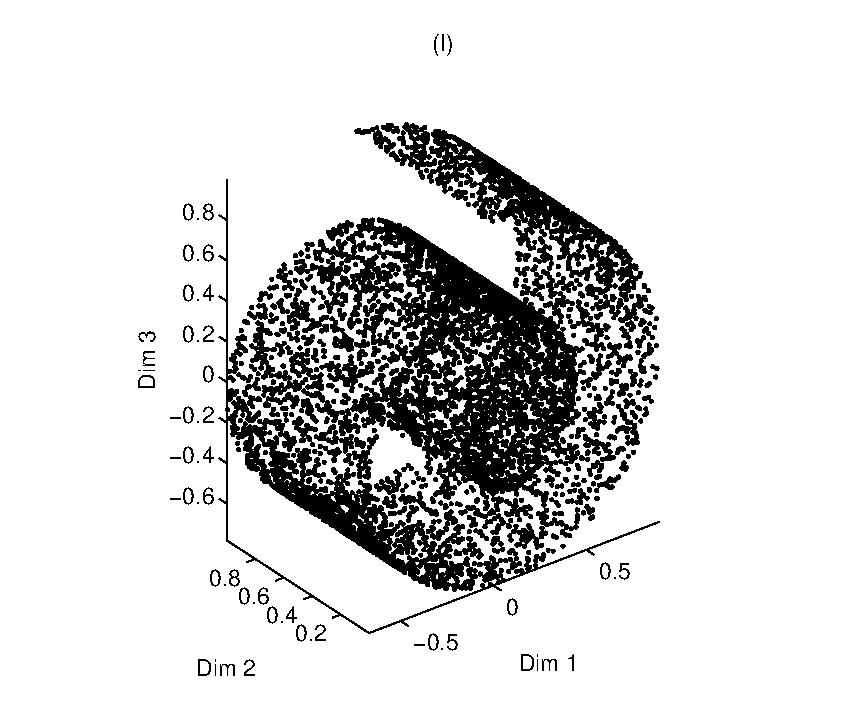
\includegraphics[width=60mm,height=50mm]{Swissroll.eps} & 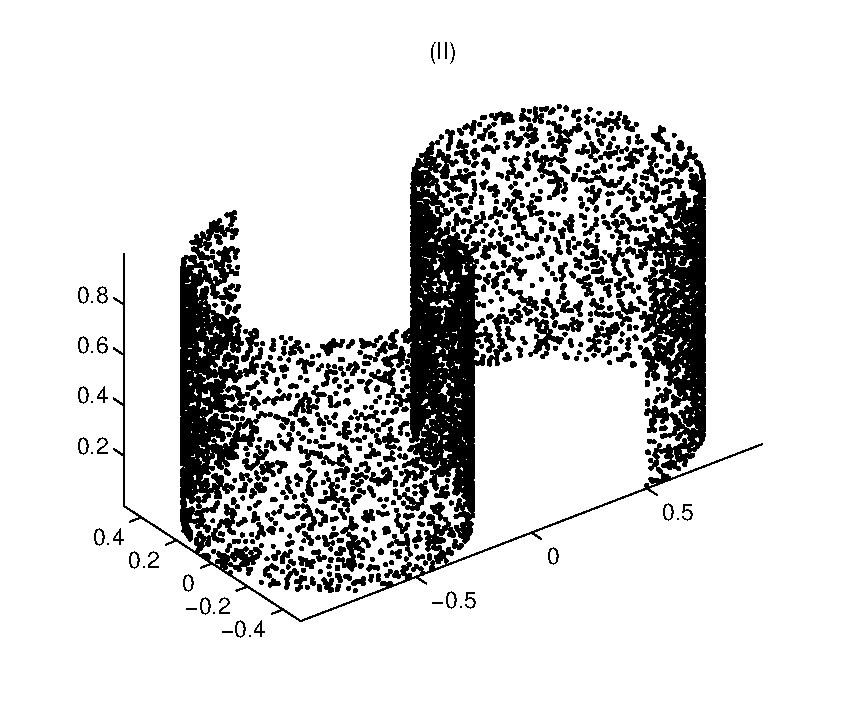
\includegraphics[width=60mm,height=50mm]{SManifold.eps}
\end{tabular}
\caption{Non-linear manifolds: Swissroll (I) and S-Manifold (II) embedded in $\mathcal{R}^3$} \label{manifold:nonlinear}
\end{figure}



\bibliographystyle{unsrt} 
\bibliography{nipsMSB_supplement} 

\end{document}

